\documentclass[a4paper,10pt]{article}
\usepackage{anysize}
\usepackage{array}
\marginsize{3cm}{3cm}{2.5cm}{2.5cm}
\usepackage[pdftex]{graphicx}

\newcommand{\analog}{\texttt{\%analog}}

\title{\%analog \\ \itshape \large
   A definitive notation for modelling \\electronic analogue computation}
\author{Charlie Care}
\date{Novemember 2004}

\begin{document}
\maketitle

\analog\ is a notation written for tkeden. 
The notation comprises of two main layers. Firstly there is the notation language itself, this was created using the agent oriented parser and is designed to provide a high-level notation for describing the relationship between the various components available on an electronic analogue computer. Secondly, there is the is the \emph{engine} that maintains the state of the computer. When \analog\ definitions are parsed, they are translated into eden definitions. This second layer consists of a number of procedures that work alongside the translated \analog\ to simulate the activity of the computer.

There is also a third layer which provides a basic grapical interface to controlling the computation. This allows \analog\ to be used for standalone simulation of an analogue computer. However, it is intended that the notation should provide a framework on which more elaborate models can be constructed and therefore this layer is not essential to the workings of the underlying notation.

\section{Analogue Computers and \%analog}
An electronic analogue computer is essentially a large set of computing components. Most of these are based on the operational amplifyer and can be configured as \emph{summers} or \emph{integrators}. Also available are various potentiometers (variable resistors) which allow variables to be scaled. As well as these components there are often function generator and multiplyers, but since these are not provided in the \analog\ notation
we will not go into them in great depth. For the purposes of the notation, summers, integrators and potentiometers are available as primitive components. The \analog\ definitions for these components are given in Table \ref{basicComponents} along with their graphical and mathematical representations.

Note that the graphical representations of the summer and integrator in \ref{basicComponents} have a the numeral $1$ next to each input and output. On an analogue computer provision is made for inputs and outputs to have an amplification factor of $1$ (no amplification) or $10$. This amplification is represented on the diagram by placing either a $1$ or a $10$ next to the relevant connection.
In \analog\ none of the connections have amplification, to represent amplified inputs and outputs you use an \texttt{amplify()} definition. 
An example is shown in Figure \ref{amplifyExample}.

\begin{figure}[h]
\center
\label{amplifyExample}
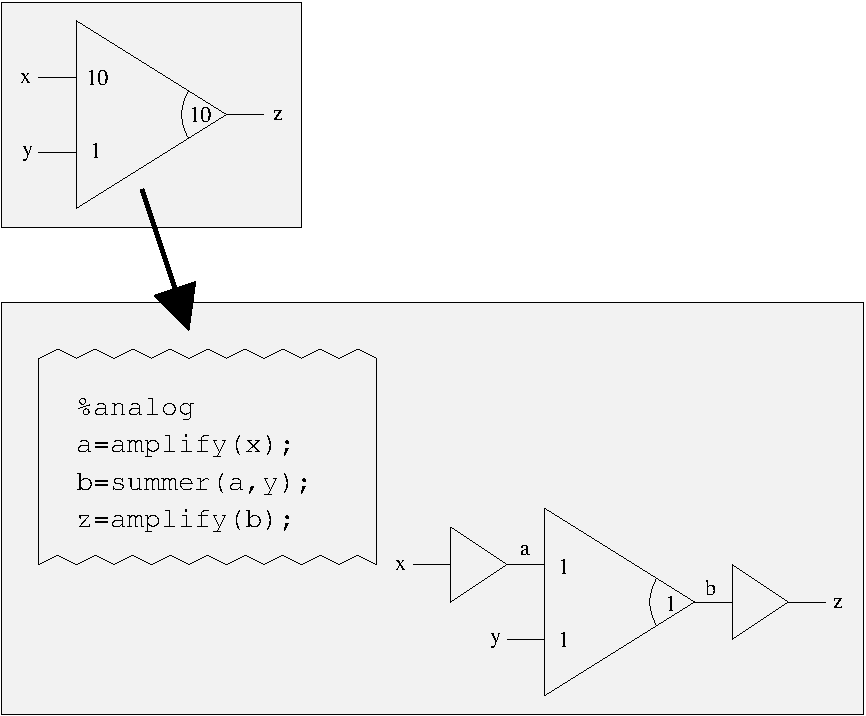
\includegraphics[width=0.5\textwidth]{amplifyExample}
\caption{How to represent amplified inputs/outputs in \analog}
\end{figure}




Sometimes, analogue integrators are shown in analogue computing diagrams with a number of inputs. Such a component is essentially a summer and an integrator in one package and is therefore reperesented in \analog\ as a summer connected to an integrator (see Figure \ref{integratorSummer}).

\begin{figure}[h]
\center
\label{integratorSummer}
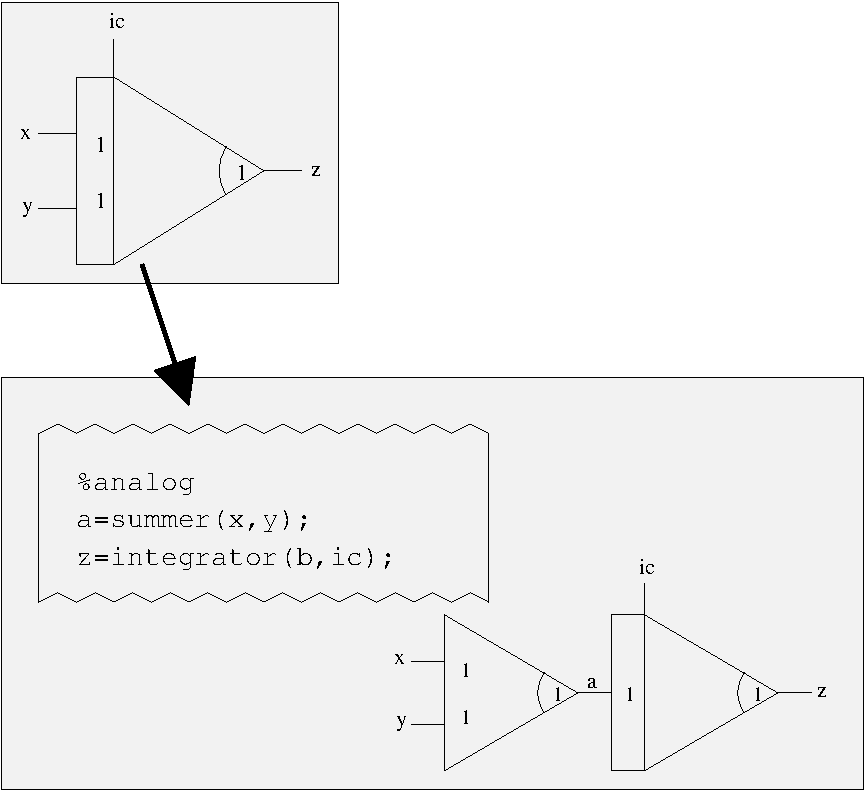
\includegraphics[width=0.5\textwidth]{integratorSummer}
\caption{How to reresent a integrator with summing inputs in \analog}
\end{figure}



\section{How to represent a differential equation}

In my copy of \cite{charlesworth} appears this example representation of 
a differential equation on an analogue computer.















\begin{table}
\label{basicComponents}
\begin{center}
\begin{tabular}{|m{40mm}|m{34mm}|m{12em}|}
\hline 
\centering Component&\centering Semantics & \ Graphical Representation\\
\hline
\hline
\centering
\begin{verbatim}
%analog
x=summer(y,z);
\end{verbatim}
  & \centering \large $x = y + z$ &  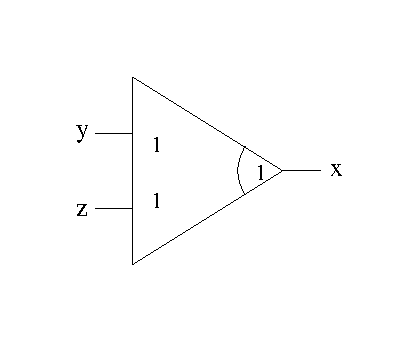
\includegraphics[width=12em]{summer}\\
\hline
\centering
\begin{verbatim}
%analog
x=integrator(ic,y);
\end{verbatim}
 & \centering \large $x= \int y dt + ic$ & 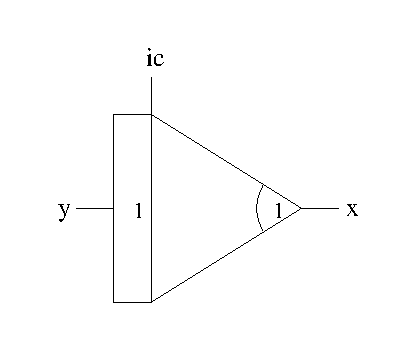
\includegraphics[width=12em]{integrator}\\
\hline
\centering
\begin{verbatim}
%analog
x=scale(0.8,y);
\end{verbatim}
 &  \centering \large $x= \frac{8}{10}y$ & 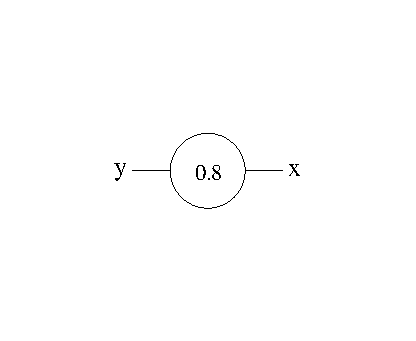
\includegraphics[width=12em]{pot}\\
 \hline
\centering
\begin{verbatim}
%analog
x=amplify(y);
\end{verbatim}
 &  \centering \large $x= 10y$ & 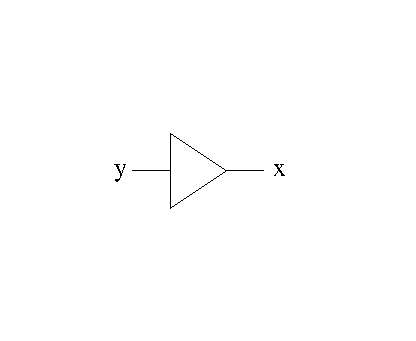
\includegraphics[width=12em]{amplify}\\
\hline
\end{tabular}
\end{center}
\caption{The basic \analog\ definitions}
\end{table}











\end{document}

\begin{}

open_panel;

mode potset;
mode reset;
mode hold;
mode compute;
mode repop;

period=123;

remove x;
forget x;

?x;
inspect x;

?*;
inspect *;

x=scale(0.9,y);
x=summer(y,z);
x=integrator(ic,y);
x=amplify(y);
x=y;

+  1 MU
- -1 MU
0  0 MU

\end{verbatim}



